\chapter{User documentation}
\label{ch:user}

This chapter documents the user-side aspects of the implemented
\emph{AI Cookbook with Ingredient-Based Search} application. It describes
how the system is prepared, configured, launched, and used in a
local thesis and development environment. It first presents the setup
and configuration steps required before the application can be used,
then documents the main workflows from the user's perspective. Because
the application integrates a FastAPI backend, a React frontend, a
local relational database, retrieval-based recipe generation, and
OCR-based nutrition label processing, proper initial setup is
required to ensure reliable execution of all workflows.

The chapter is organized into three sections. Section 2.1 outlines
the technical prerequisites and configuration steps, including
hardware and software requirements, dependency installation,
environment variables, and initial verification. Section 2.2
provides a user manual describing the main workflows, such as
recipe generation, personalization features, recipe storage, and
OCR-based food label extraction. Section 2.3 discusses known
issues, system limitations, and frequently asked questions based
on practical usage.

\cleardoublepage


\section{Installation, setup, and configuration guide}

This section describes the requirements and steps necessary to run
the application in a local development environment. It covers the
hardware and software prerequisites, required external services,
and the configuration steps needed before the backend, frontend,
database, vector store, and AI-supported features can be used.

\subsection{System requirements}

This subsection defines the conditions that should be satisfied
before the application is installed and executed in a local
development environment. Because the system combines a Python-based
backend, a React frontend, local persistent storage, and
multiple AI-supported services, successful operation depends on both
local development tools and external API access. The requirements
are therefore grouped into three categories: hardware requirements,
software requirements, and external service requirements.

\subsubsection{Hardware requirements}

\begin{itemize}
	\item \textbf{Operating system:} Windows~10 or newer, a recent Linux
	distribution, or a recent macOS version.
	\item \textbf{Processor:} Any modern 64-bit multi-core processor is
	sufficient for development and local execution.
	\item \textbf{Memory (RAM):} At least 8~GB is required, while 16~GB is
	recommended for smoother use when the backend, frontend, browser,
	and indexing-related tasks are active at the same time.
	\item \textbf{Storage:} At least 4~GB of free disk space is
	recommended. This covers the project source code, Python and Node.js
	dependencies, the local SQLite database, uploaded OCR images,
	generated recipe thumbnails, and the persisted Chroma vector store.
	\item \textbf{Internet connection:} Required during both setup and
	normal use. Dependency installation requires network access, and the
	AI-supported workflows depend on external APIs for recipe generation,
	embedding generation, OCR processing, and nutrition-data
	structuring.
\end{itemize}

\subsubsection{Software requirements}

\begin{itemize}
	\item \textbf{Python 3.11 or newer.} Required for the FastAPI backend,
	virtual environment management, dependency installation, Alembic
	database migrations, recipe indexing scripts, and backend testing.

	Download: \url{https://www.python.org/downloads/}.
	\item \textbf{Node.js and npm.} Required for installing frontend
	dependencies and running the React application through the Vite
	development server. A recent LTS version is recommended for local
	development.

	Download: \url{https://nodejs.org/en/download}.
	\item \textbf{Git.} Recommended for cloning, updating, and managing
	the repository in a reproducible way.

	Installation guide:\\
	\url{https://git-scm.com/book/en/v2/Getting-Started-Installing-Git}.
	\item \textbf{Modern web browser.} Required to access the frontend
	locally. Google Chrome, Mozilla Firefox, and Microsoft Edge are all
	suitable for development and normal use.
\end{itemize}

For platform-specific Python installation, interpreter usage, and
environment-management details, the official \emph{Python Setup and
Usage} guide can be consulted \cite{python2026setup}.

For platform-specific Node.js and npm installation details, the
official Node.js installation guide can be consulted
\cite{node2026setup}.

\subsubsection{External service requirements}

In addition to the local software stack, the AI-supported features
require access to two external services. The application can start
without these credentials, but the affected AI-supported workflows
will not function correctly until they are configured.

\textbf{OpenAI API access} is required for recipe generation,
embedding generation for the retrieval pipeline, structuring
OCR-extracted nutrition data into JSON, producing nutritional
estimates for generated recipes, and generating recipe thumbnail
images. For full local deployment, the application expects a valid
OpenAI API key to be provided through environment configuration by
the maintainer or developer operating the system. Ordinary end
users do not enter this value through the application interface.
Further information is
available at:
\par{\footnotesize\url{https://help.openai.com/en/articles/4936850-where-do-i-find-my-openai-api-key}}

\textbf{Google Cloud Vision credentials} are required for
OCR-based nutrition label extraction. The application expects
credentials to be provided through the
\texttt{GOOGLE\_APPLICATION\_CREDENTIALS} environment variable,
following the standard Google Cloud authentication flow. As with the
OpenAI key, these credentials are supplied during environment setup
by the maintainer or developer rather than by ordinary end users.
The authentication setup is described at:
\par
\url{https://cloud.google.com/vision/docs/authentication}.

\subsection{Getting the source code and installing dependencies}

This subsection explains how the project is obtained and how the
development dependencies are prepared for first use. The repository
contains a Python backend, a React frontend, migration files,
testing material, and thesis-related assets, so the complete project
root should be available locally before configuration begins.

The source code is hosted in a Git repository. Cloning the repository
is the preferred approach because it preserves the full project
structure and allows future updates to be pulled in a consistent way.
If the project is already available locally as a thesis submission
archive or extracted folder, the same setup steps can be followed from
that project root without cloning again.
The repository can be obtained with the following commands:

\lstset{caption={Cloning the project repository}, label=src:user-get-repo}
\begin{lstlisting}
git clone https://github.com/ulkarchbnv/ai-cookbook-thesis.git
cd ai-cookbook-thesis
\end{lstlisting}

After cloning, the project root should contain the main application
directories used during setup and development, most importantly
\texttt{backend}, \texttt{frontend}, \texttt{alembic}, and
\texttt{docs}. The
\texttt{backend} directory contains the FastAPI application and its
service logic, the \texttt{frontend} directory contains the React user
interface, and the \texttt{alembic} directory contains the database
migration files used to initialize and update the local schema. The
\texttt{docs} directory contains testing and evaluation material used
elsewhere in the thesis.

After the repository has been cloned, the backend environment should
be prepared first. The application uses Python for the backend, so it
is recommended to create a dedicated virtual environment in the
project root. This avoids interference with globally installed Python
packages and keeps the local setup reproducible.

\lstset{caption={Creating the Python virtual environment}, label=src:user-create-venv}
\begin{lstlisting}
python -m venv .venv
\end{lstlisting}

On Windows PowerShell, the virtual environment can be activated as
follows:

\lstset{caption={Activating the virtual environment in PowerShell}, label=src:user-activate-venv-win}
\begin{lstlisting}
.\.venv\Scripts\Activate.ps1
\end{lstlisting}

On Linux or macOS shells, the typical activation command is:

\lstset{caption={Activating the virtual environment on Linux or macOS}, label=src:user-activate-venv-unix}
\begin{lstlisting}
source .venv/bin/activate
\end{lstlisting}

Once the virtual environment is active, the backend requirements can
be installed from the dependency list stored in
\texttt{backend/requirements.txt}. This step installs the web
framework, database and migration libraries, AI-service client
libraries, OCR-related packages, retrieval-pipeline dependencies, and
project support tools such as the backend testing framework.

\lstset{caption={Installing backend dependencies}, label=src:user-install-backend}
\begin{lstlisting}
python -m pip install --upgrade pip
python -m pip install -r backend/requirements.txt
\end{lstlisting}

At this point, the backend runtime, database libraries, migration
tools, OCR-related dependencies, AI client libraries, and testing
packages are available inside the local virtual environment.

The frontend is maintained separately in the \texttt{frontend}
directory and must also be initialized before the application can be
started. Its dependencies are installed with \texttt{npm}, which
downloads the packages required for the React user interface, routing,
the Vite development server, and frontend tests.

\lstset{caption={Installing frontend dependencies}, label=src:user-install-frontend}
\begin{lstlisting}
cd frontend
npm install
cd ..
\end{lstlisting}

After both installation steps have finished, the local machine
contains all project files and package dependencies needed for the
next stage of setup. The environment is then ready for configuration
of the variables used by the backend and frontend services, which is
described in the following subsection.

\subsection{Environment configuration}

After the repository and package dependencies have been prepared, the
next step is to define the environment variables required by the
application. The backend loads its configuration from a
\texttt{.env} file located in the project root. The frontend reads its
API base URL through Vite environment handling, and in the current
implementation it also falls back to
\texttt{http://127.0.0.1:8000} when \texttt{VITE\_API\_BASE\_URL} is
not explicitly provided.

The project already provides a template file named
\texttt{.env.example}. This file should be copied to a new file named
\texttt{.env}, and the placeholder values should then be replaced
with valid local configuration values.

\lstset{caption={Creating the local environment file}, label=src:user-create-env}
\begin{lstlisting}
copy .env.example .env
\end{lstlisting}

On Linux or macOS, the equivalent command is typically:

\lstset{caption={Creating the local environment file on Linux or macOS}, label=src:user-create-env-unix}
\begin{lstlisting}
cp .env.example .env
\end{lstlisting}

The most important variables for local execution are the following:

\begin{itemize}
	\item \textbf{\texttt{OPENAI\_API\_KEY}} specifies the API key used by
	the recipe-generation, embedding, nutrition-structuring, and image
	generation features.
	\item \textbf{\texttt{GOOGLE\_APPLICATION\_CREDENTIALS}} points to the
	local path of the Google Cloud service-account JSON file used by the
	OCR provider.
	\item \textbf{\texttt{DATABASE\_URL}} defines the relational database
	connection. If this value is not overridden, the backend defaults to
	a local SQLite database file named \texttt{ai\_cookbook.db} in the
	project root.
	\item \textbf{\texttt{SECRET\_KEY}} is required for JWT creation and
	validation and must not be left empty.
	\item \textbf{\texttt{FRONTEND\_ORIGIN}} defines the allowed frontend
	origin for backend CORS handling. In the default local setup, this
	should match the Vite development server address.
\end{itemize}

In addition to these core values, the configuration file also
contains optional settings for model names, retrieval parameters,
upload limits, media directories, rate-limiting rules, and vector
store persistence paths. Many of these defaults are already suitable
for a standard local development setup, so they do not need to be
changed unless the deployment environment or experimental requirements
differ from the default configuration. However, required values such
as \texttt{SECRET\_KEY}, \texttt{OPENAI\_API\_KEY}, and, for OCR
usage, \texttt{GOOGLE\_APPLICATION\_CREDENTIALS}, must still be
configured explicitly.

If the frontend should target a backend address other than the default
\texttt{http://127.0.0.1:8000}, the \texttt{VITE\_API\_BASE\_URL}
variable can be provided through the frontend's Vite environment
configuration.

A typical local \texttt{.env} file follows the structure shown in
Code~\ref{src:user-env-example}. The values below are examples only
and should be replaced with valid credentials and paths. The example
is intentionally limited to the most important backend settings for a
standard local setup.

\lstset{caption={Example local environment configuration}, label=src:user-env-example}
\begin{lstlisting}
OPENAI_API_KEY=your_openai_key
OCR_PROVIDER=google_vision
GOOGLE_APPLICATION_CREDENTIALS=C:\path\to\your-google-service-account.json
DATABASE_URL=sqlite:///./ai_cookbook.db
SECRET_KEY=your_secret_key
ALGORITHM=HS256
FRONTEND_ORIGIN=http://localhost:5173
\end{lstlisting}

When this file has been created and updated, the backend can load its
runtime settings correctly, and the frontend can target the intended
local API endpoint.

\subsection{Verifying the installation}

Before launching the application, it is useful to verify that the
main tools and local files are available as expected. This helps
detect common setup mistakes early, such as a missing virtual
environment, an unavailable Node.js installation, or an incorrectly
named configuration file.

The first check is to confirm that the required command-line tools
are accessible and return valid version information.

\lstset{caption={Verifying the local toolchain}, label=src:user-verify-toolchain}
\begin{lstlisting}
python --version
node --version
npm --version
git --version
\end{lstlisting}

At this stage, Python should report version 3.11 or newer, while
Node.js and npm should also return installed versions without error.
Git is not required for runtime execution after cloning, but it
should still be available if the repository will be updated or
maintained locally.

The second check is to confirm that the expected local setup artifacts
exist in the project root. In a correctly prepared environment, the
repository should already contain the application source directories,
the \texttt{.venv} virtual environment directory, and the
\texttt{.env} configuration file.

\lstset{caption={Verifying key local files and directories}, label=src:user-verify-files}
\begin{lstlisting}
Get-ChildItem .venv, backend, frontend, alembic, .env
\end{lstlisting}

If these files and directories are present, the local installation can
be considered structurally complete. The next step is to initialize
the database and other local data resources required by the
application.

\subsection{Initializing the database and local retrieval data}

After the installation has been verified, the local data layer should
be initialized. In the default configuration, the backend uses a
SQLite database defined through \texttt{DATABASE\_URL}, and its schema
is managed through Alembic migration files located in the
\texttt{alembic} directory. Running the migration step ensures that
the required tables and indexes are created before the application is
started.

The migration command should be executed from the project root while
the Python virtual environment is active:

\lstset{caption={Applying database migrations}, label=src:user-run-migrations}
\begin{lstlisting}
alembic upgrade head
\end{lstlisting}

When this command completes successfully, the local database schema
contains the tables required for users, generated recipes, and saved
OCR extraction history. In the default SQLite-based setup, the file
\texttt{ai\_cookbook.db} is created automatically in the project root
if it does not already exist.

In addition to the relational database, the recipe-generation workflow
also depends on local retrieval data. The project already includes a
prepared recipe subset in \texttt{backend/data/recipes\_subset.json},
which serves as the source corpus for the retrieval-augmented
generation pipeline. This subset was prepared from the Food.com dataset
distributed through Kaggle. To make this corpus searchable, it must be
embedded and indexed into the local Chroma vector store.

\lstset{caption={Indexing the recipe corpus for retrieval}, label=src:user-index-recipes}
\begin{lstlisting}
python -m backend.scripts.index_recipes
\end{lstlisting}

This step reads the recipe subset, generates embeddings for the recipe
documents, and stores them in the Chroma persistence directory
specified by \texttt{CHROMA\_PERSIST\_DIRECTORY}. It should be executed
at least once before recipe generation is tested on a new local setup.

The project also includes a preparation script that can regenerate the
cleaned recipe subset when the raw dataset is available locally. For
normal local setup, however, this preprocessing step is not required
because the prepared subset used by the application is already
included in the repository.

Once the database migrations and vector-store indexing have both been
completed, the system is ready to launch the backend and frontend
services.

\subsection{Starting the backend and frontend}

After the local data layer has been initialized, the application can
be started. The backend and frontend run as separate development
services, so they are typically launched in two terminal windows.

The backend should be started first from the project root while the
Python virtual environment is active:

\lstset{caption={Starting the FastAPI backend}, label=src:user-start-backend}
\begin{lstlisting}
uvicorn backend.main:app --reload
\end{lstlisting}

In the default local configuration, the backend starts on
\texttt{http://127.0.0.1:8000}. If the startup is successful, the
terminal displays the Uvicorn server message and begins watching the
project files for code changes.

If a different host or port is needed, or if the backend must later be
deployed behind HTTPS with an SSL certificate, these operational details
should be taken from the official FastAPI deployment guide rather than
duplicated here \cite{fastapi2026deployment}.

The frontend is started separately from the \texttt{frontend}
directory:

\lstset{caption={Starting the React frontend}, label=src:user-start-frontend}
\begin{lstlisting}
cd frontend
npm run dev
\end{lstlisting}

In the default setup, the Vite development server starts on
\texttt{http://localhost:5173}. The frontend sends its API requests to
the backend URL defined by \texttt{VITE\_API\_BASE\_URL}, which should
therefore match the backend address used during startup.

When both services are running, the application can be opened in a web
browser by visiting the frontend address. The backend exposes the API
used by the user interface, while the frontend provides access to the
pages for recipe generation, nutrition label extraction, saved items,
history, and account management.

\subsection{Post-startup verification}

After both services have been started, a short smoke test should be
performed before the full user workflows are exercised. The purpose of
this check is not detailed feature validation, but quick confirmation
that the local setup is operational.

The backend can be checked by opening
\texttt{http://127.0.0.1:8000/} in a browser. In a successful setup,
the service returns a small JSON response containing the message
\texttt{"AI Cookbook backend is running"}.

The frontend can be checked by opening
\texttt{http://localhost:5173}. In a successful setup, the home page
of the application is displayed and the main navigation bar is visible.
It should then be possible to open the \textbf{Generate} and
\textbf{Food Labels} pages without an immediate runtime error.

Once this smoke test succeeds, the local setup can be considered
complete and the application is ready for functional use. The
following section describes the user workflows supported by the
system.

\section{User manual}

This section describes how the application is used after the local
environment has been configured and both services are running. The
manual covers both the first-use path through the application and the
main workflows available from the implemented user interface. It is
based on the actual frontend structure of the system and focuses on
the features that are most important from the user perspective:
accessing the system, managing an account, generating recipes,
processing food labels, and reviewing saved or historical results.

Although recipe generation can be used without authentication,
creating an account unlocks the persistence features of the system.
Authenticated users can store dietary preferences and allergy
defaults, save generated recipes, and keep a history of both recipe
generation and OCR-based food label extraction.

\subsection{Quick-start walkthrough from launch to first meaningful action}

This subsection provides a short first-use path through the
application. Its purpose is to help a new evaluator or user reach a
meaningful result quickly after startup, without yet exploring every
feature in detail.

Once the backend and frontend have been started as described in the
previous section, the application is opened at
\texttt{http://localhost:5173}. The home page appears first and gives
access to the two main workflows of the system: recipe generation and
food-label extraction.

The quickest meaningful action is recipe generation as a guest user.
The user opens the \textbf{Generate} page, enters a comma-separated
list of ingredients such as \texttt{chicken, rice, onion}, and submits
the form with the \textbf{Generate Recipe} button. If the backend is
configured correctly and the required AI services are available, the
page returns a structured recipe containing a title, ingredients,
preparation steps, a nutrition estimate, and any warning messages.
This confirms that the main backend, retrieval, and frontend response
flow is operational.

An alternative first-use path is the OCR-based workflow. The user
opens the \textbf{Food Labels} page, selects an image of a nutrition
label, and clicks \textbf{Extract Nutrition}. A successful response
returns both raw OCR text and structured nutrition data. This confirms
that file upload, OCR processing, and AI-assisted structuring are all
working.

If the user wants to test persistence features as part of the initial
exploration, the next step is to open the \textbf{Login} page, create
an account, and log in. After authentication, generated recipes can be
saved, profile defaults can be configured, and recipe or OCR history
becomes available.

\subsection{Feature-by-feature guide with annotated key screens}

This subsection presents the main screens of the implemented user
interface one by one. Each screenshot is accompanied by a short
textual annotation describing the most important visible areas and the
user actions supported on that screen.

\subsubsection{Home page and basic navigation}

When the frontend is opened in the browser, the application displays
the home page. This page functions as the main entry point and gives
the user a concise overview of the system. It introduces the three
main capabilities of the application: recipe generation,
OCR-supported nutrition label extraction, and data persistence.

The page also provides two primary call-to-action buttons:

\begin{itemize}
	\item \textbf{Generate a Recipe}, which opens the recipe-generation
	page.
	\item \textbf{Scan a Food Label}, which opens the OCR-based nutrition
	label page.
\end{itemize}

At the top of the interface, the navigation bar provides access to the
main pages of the system:

\begin{itemize}
	\item \textbf{Home} returns to the landing page.
	\item \textbf{Generate} opens the recipe-generation workflow.
	\item \textbf{Food Labels} opens the nutrition label extraction page.
	\item \textbf{Saved} displays recipes that have been explicitly saved
	by the authenticated user.
	\item \textbf{History} displays the user's generated recipe history,
	including unsaved entries.
	\item \textbf{Login} or \textbf{Account} opens the authentication and
	profile-management page.
\end{itemize}

If the user is already authenticated, the navigation bar also displays
a \textbf{Logout} button. This immediately removes the stored session
token on the client side and returns the application to guest mode.

The main visible areas of the screen are the headline section, the two
primary action buttons, and the top navigation bar. Together, these
elements guide the user toward either the recipe-generation or OCR
workflow and provide access to the rest of the application. This layout
is shown in Figure~\ref{fig:user-home-page}.

\begin{figure}[H]
	\centering
	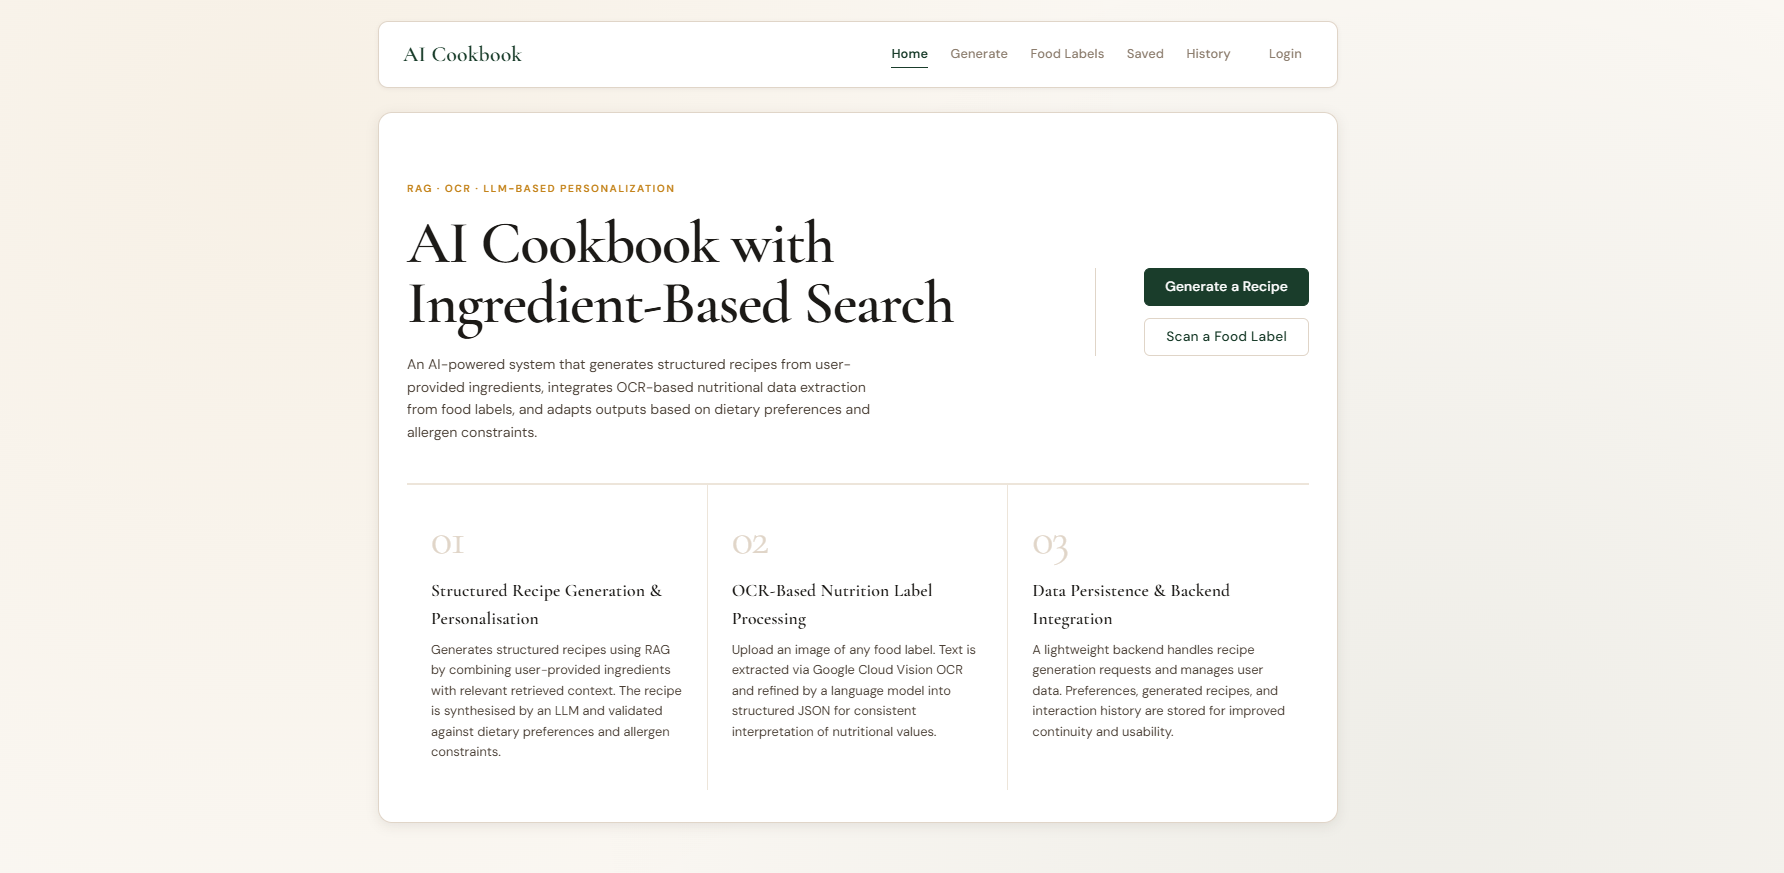
\includegraphics[width=0.9\textwidth]{images/HomePage.png}
	\caption{Home page of the AI Cookbook application}
	\label{fig:user-home-page}
\end{figure}

\subsubsection{Account creation, login, and profile defaults}

The \texttt{/login} page serves both as the authentication page for
guest users and as the account-management page for authenticated
users. Before login, the page presents two tabs: \textbf{Login} and
\textbf{Sign Up}. This allows a new user to create an account without
leaving the page. The guest-facing authentication view is shown in
Figure~\ref{fig:user-login-page}.

\begin{figure}[H]
	\centering
	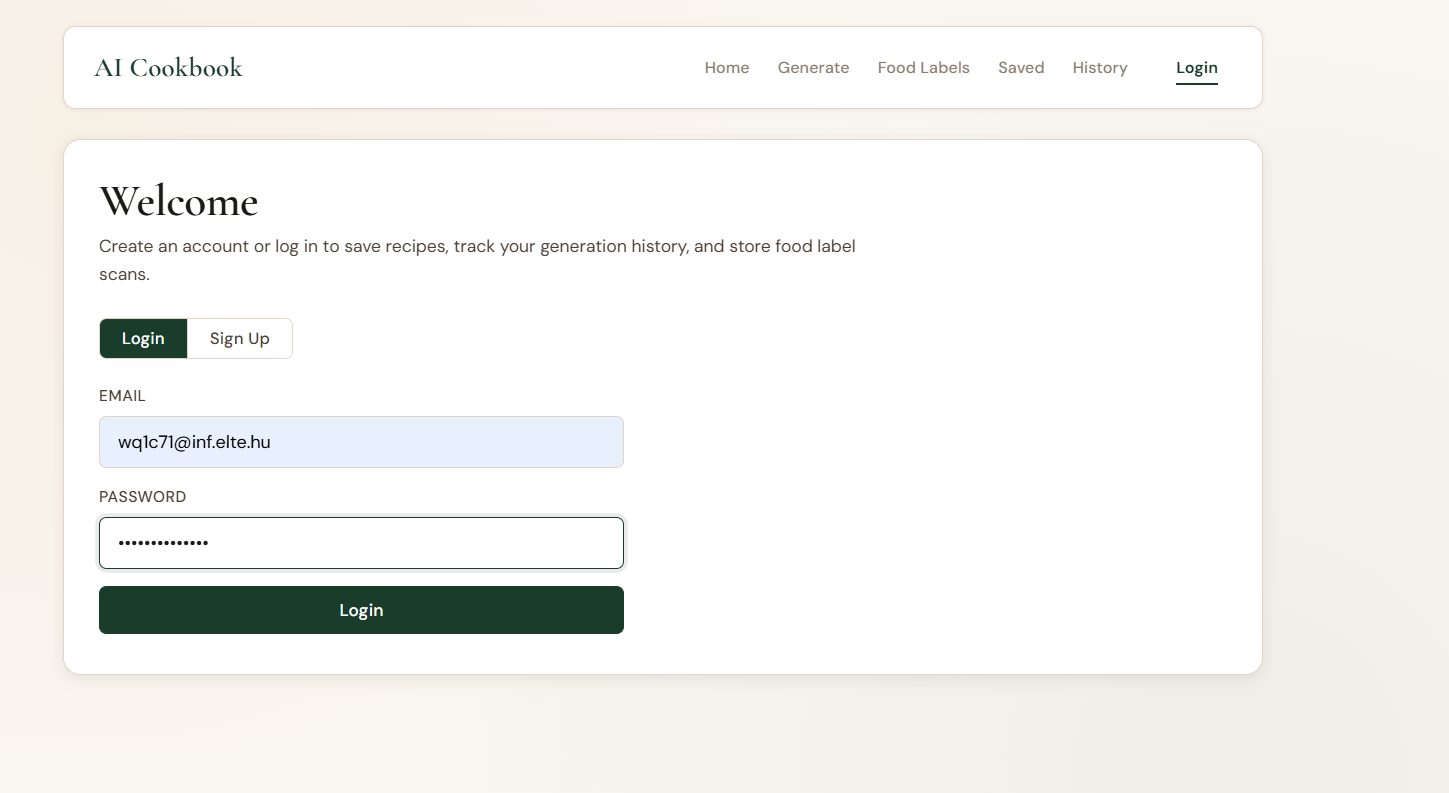
\includegraphics[width=0.82\textwidth]{images/Login.png}
	\caption{Login and registration page}
	\label{fig:user-login-page}
\end{figure}

To register a new account, the user switches to the \textbf{Sign Up}
tab, enters an email address and password, and submits the form. If
the email address is not already registered, the system creates the
account and returns a confirmation message. The user can then switch
back to the login tab and authenticate with the same credentials.

To log in, the user enters the registered email address and password
and submits the login form. On successful authentication, the backend
returns a JWT access token. The frontend stores this token locally and
uses it automatically in subsequent authenticated requests.

After login, the same page changes into an account-management view.
Instead of the login form, the user sees a summary of the current
profile data:

\begin{itemize}
	\item the account email address,
	\item the saved list of dietary preferences,
	\item the saved list of allergies.
\end{itemize}

Below the profile summary, the page provides a form for updating
default dietary preferences and allergy values. These defaults are
important because they can be reused later on the recipe-generation
page. If the user leaves the optional preference and allergy fields
empty during recipe generation, the application automatically falls
back to the saved profile values.

This makes the account page an important bridge between authentication
and later personalized recipe-generation behavior, because the values
stored here directly affect future requests when the user relies on
saved defaults.

The key visible parts of this screen are the tab selector, the
credential form, and, after login, the profile summary and update
form. This page therefore functions both as the entry point for
authentication and as the place where personalization defaults are
maintained. The authenticated account-management view is shown in
Figure~\ref{fig:user-account-page}.

\begin{figure}[H]
	\centering
	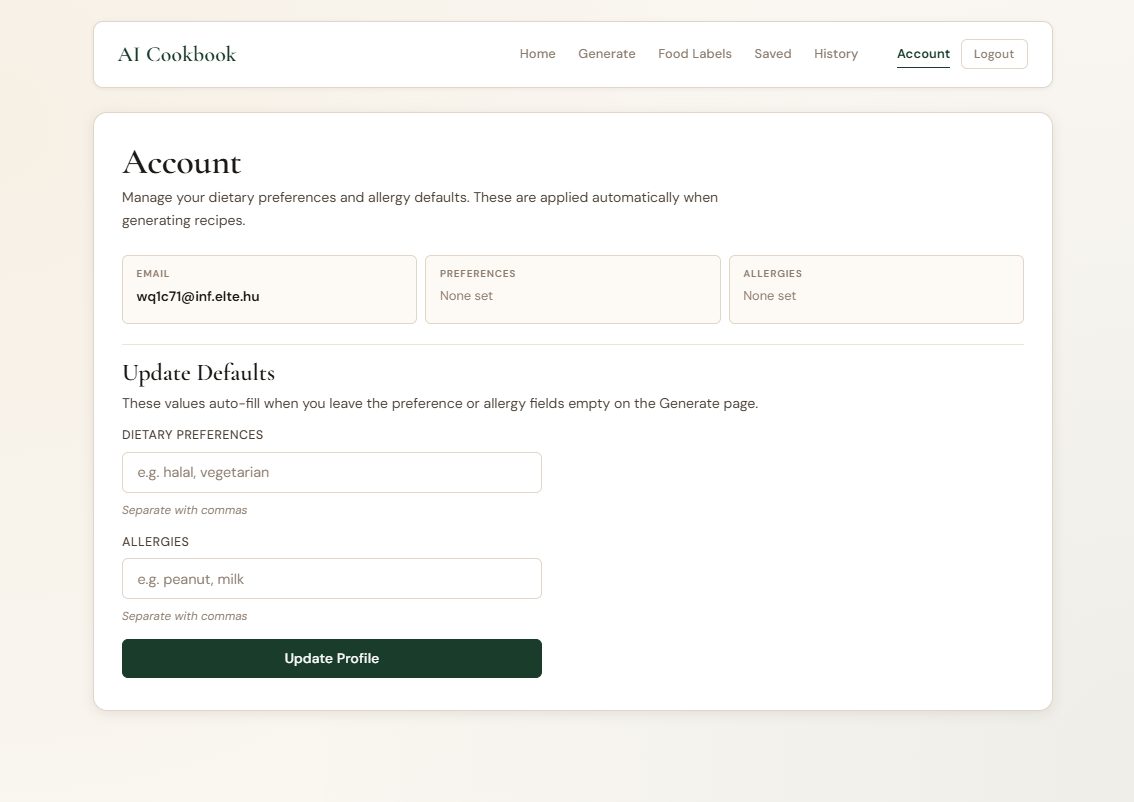
\includegraphics[width=0.82\textwidth]{images/Account.png}
	\caption{Account page after login, showing saved dietary defaults}
	\label{fig:user-account-page}
\end{figure}

\subsubsection{Recipe generation}

The recipe-generation page is the main workflow of the application.
The user enters a comma-separated list of available ingredients and
may optionally specify dietary preferences and allergies. If the user
is already authenticated and has saved default preferences or allergy
values in the account page, these defaults are applied automatically
when the optional fields are left empty.

After the form is submitted, the frontend sends the request to the
backend recipe-generation endpoint. The backend validates the input,
retrieves relevant recipe context from the indexed corpus, invokes the
language model, and returns a structured response. The result page
shows the generated recipe title, ingredient list, any additional
ingredients that may be required, preparation steps, a nutrition
estimate, and warning messages where applicable.

The screen is organized around three main areas: the input form, the
recipe result card, and the save action shown for authenticated users.
This makes it possible to move directly from ingredient entry to
inspection of the returned recipe and, when logged in, to persistence
of the result. The implemented screen is shown in
Figure~\ref{fig:user-generate-recipe}.

If the recipe was generated while the user was logged in, the page
also offers a \textbf{Save Recipe} action. This stores the generated
recipe in the user's saved collection and also preserves it in the
generation history.

\begin{figure}[H]
	\centering
	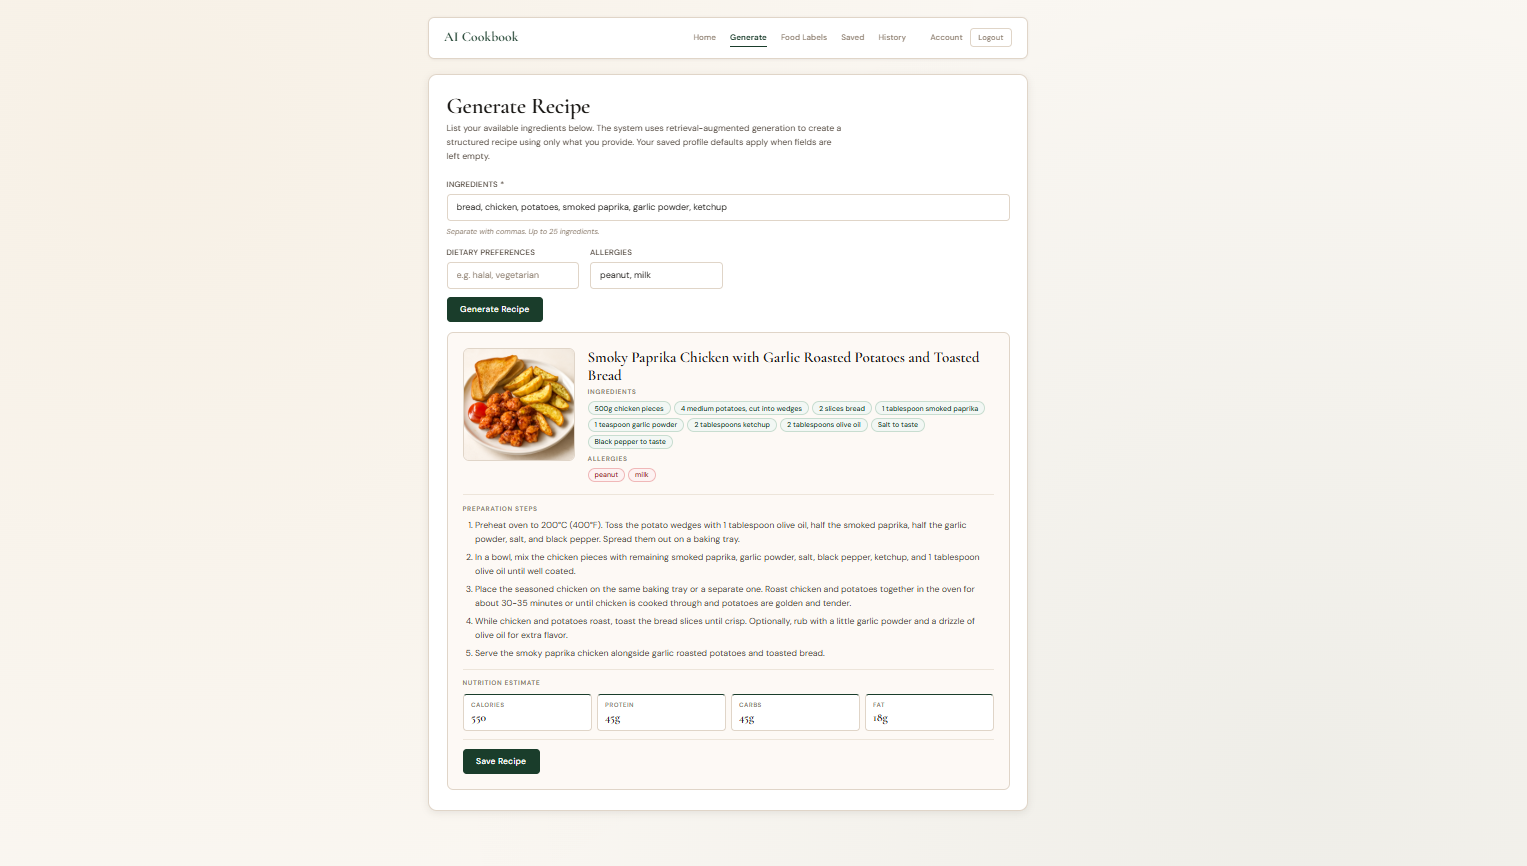
\includegraphics[width=0.9\textwidth]{images/GenerateRecipe.png}
	\caption{Recipe-generation page with a generated result}
	\label{fig:user-generate-recipe}
\end{figure}

\subsubsection{Food label extraction}

The \textbf{Food Labels} page provides the OCR-based nutrition-label
workflow. The user selects an image file containing a food label and
submits it for processing. The page first shows a local preview of the
selected image, then displays the extracted structured nutrition
values together with the raw OCR text returned by the backend.

If the user is logged in, the extracted result can be saved to the
personal label history. Saved entries remain available on the same
page and can be browsed with pagination when multiple records exist.
For unauthenticated users, extraction is still available, but
persistent storage is disabled.

The main visible regions on this page are the upload area, the
extraction result block, and the saved label history shown for
authenticated users. This page therefore combines immediate OCR usage
with later review of previously saved extraction results. The screen is
shown in Figure~\ref{fig:user-ocr-page}.

\begin{figure}[H]
	\centering
	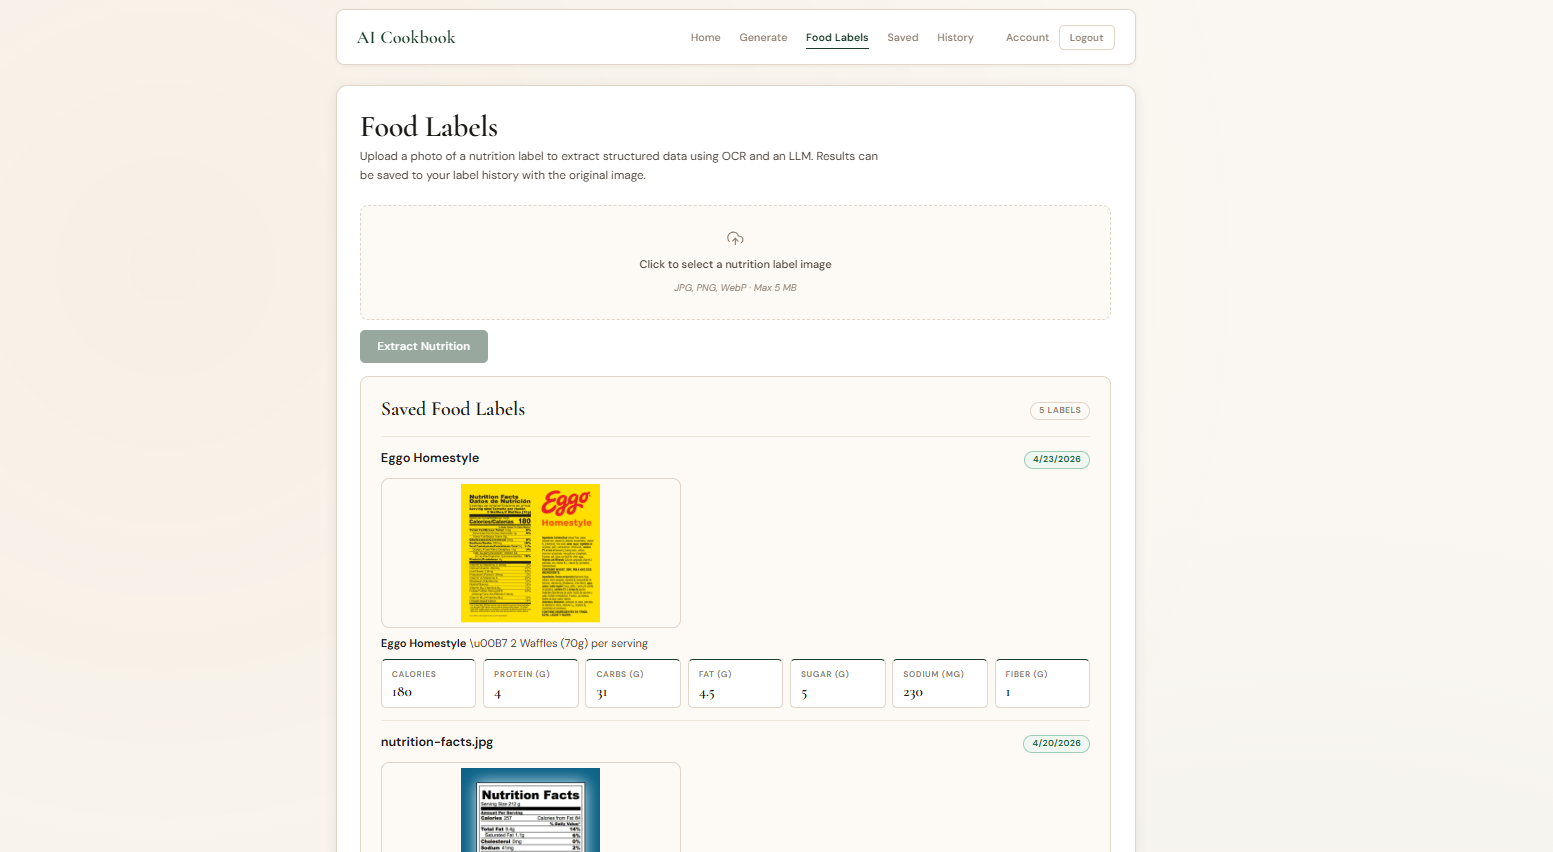
\includegraphics[width=0.9\textwidth]{images/OCR.png}
	\caption{Food label extraction page with OCR result}
	\label{fig:user-ocr-page}
\end{figure}

\subsubsection{Saved recipes}

The \textbf{Saved} page lists recipes that the authenticated user has
explicitly bookmarked after generation. Each entry is displayed as a
card containing the recipe title, key ingredients, optional
preferences and allergy markers, and the date on which the recipe was
saved.

The cards can be expanded interactively to reveal the preparation
steps and nutrition estimate. If the user is not logged in, the page
does not display private content and instead instructs the visitor to
authenticate first.

The key visible elements are the list of saved recipe cards, the saved
date indicator, and the expandable details section. This keeps the
page focused on compact review first and detailed inspection only when
requested by the user. The page is shown in
Figure~\ref{fig:user-saved-recipes}.

\begin{figure}[H]
	\centering
	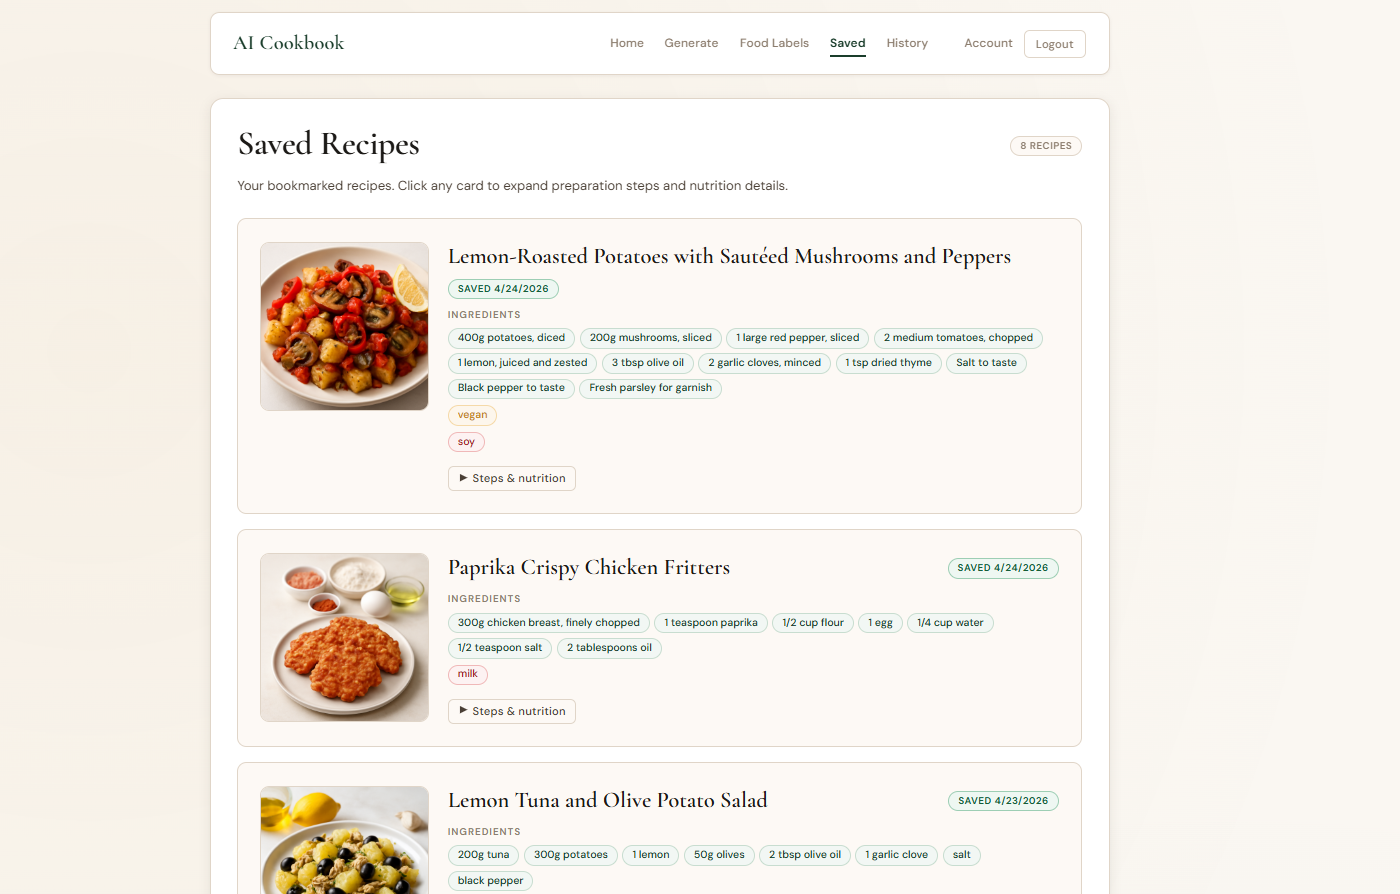
\includegraphics[width=0.9\textwidth]{images/SavedRecipes.png}
	\caption{Saved recipes page}
	\label{fig:user-saved-recipes}
\end{figure}

\subsubsection{Recipe history}

The \textbf{History} page provides a broader view than the saved
recipes page. It includes every recipe generated by the authenticated
user, including entries that were not explicitly saved. This makes the
page useful for reviewing previous outputs, comparing generated
results, and returning to earlier recipe ideas.

Each history card shows whether the recipe is merely generated or also
saved, along with the creation timestamp and any warning messages
returned during generation. As on the saved recipes page, each card
can be expanded to display the preparation steps and nutrition
estimate in full detail.

The visible structure of the page emphasizes recipe status, creation
time, and warning information, so that the user can distinguish
quickly between temporary and explicitly saved outputs before opening
the full details. The page is shown in
Figure~\ref{fig:user-recipe-history}.

\begin{figure}[H]
	\centering
	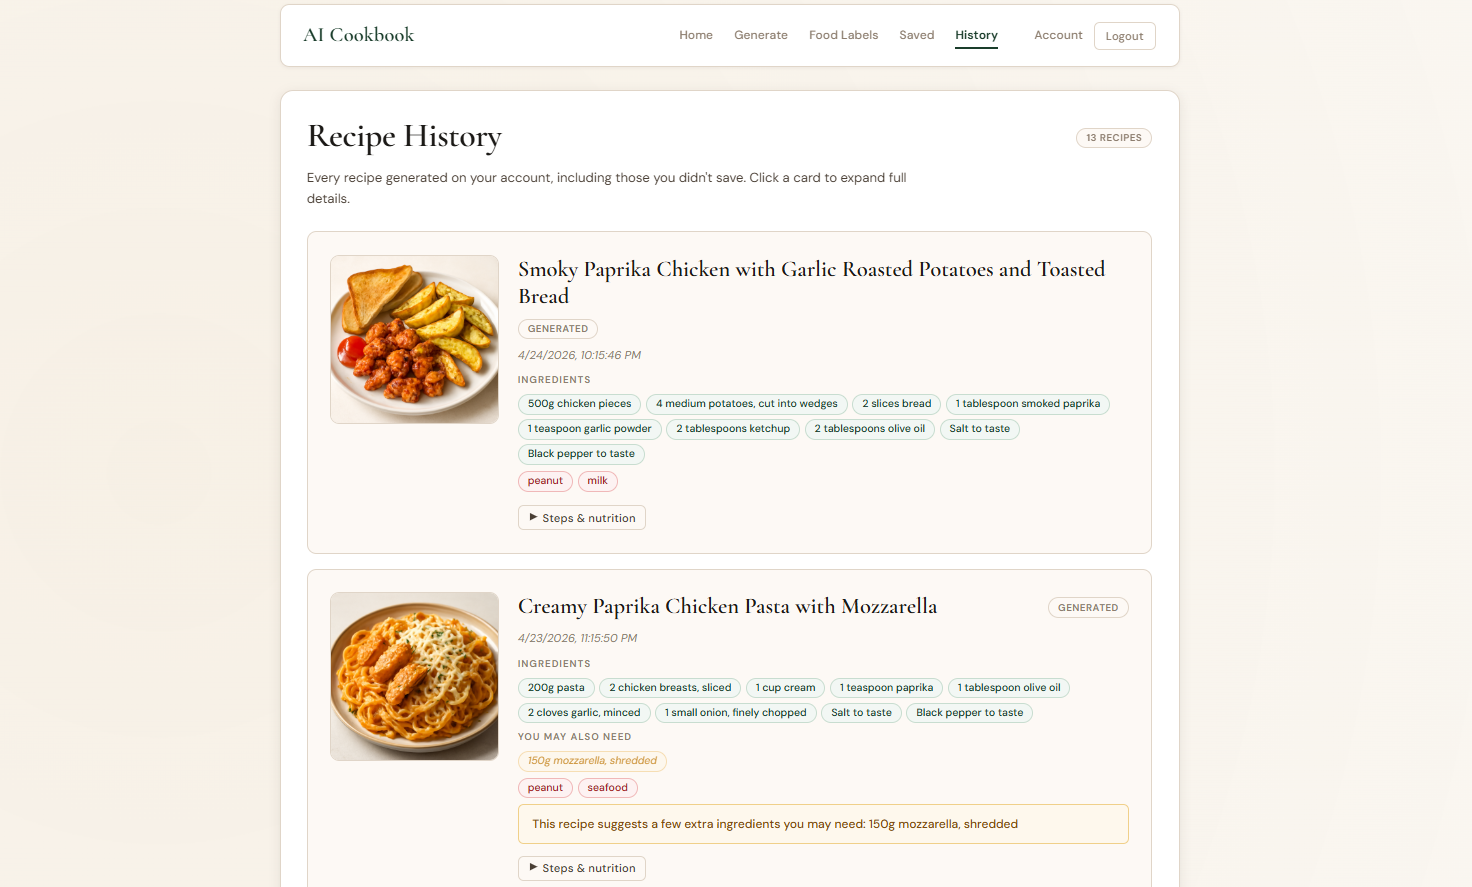
\includegraphics[width=0.9\textwidth]{images/History.png}
	\caption{Recipe history page}
	\label{fig:user-recipe-history}
\end{figure}

\subsection{Step-by-step workflows for the main features}

This subsection collects the most important multi-step workflows of the
application in a task-oriented format. These workflows correspond to
the main interactive features promised by the project and implemented
in the final system.

\subsubsection{Creating an account and setting profile defaults}

\begin{enumerate}
	\item Open the \textbf{Login} page from the navigation bar.
	\item Select the \textbf{Sign Up} tab.
	\item Enter a valid email address and password, then submit the form.
	\item Return to the \textbf{Login} tab and authenticate with the same
	credentials.
	\item After login, review the account summary shown on the same page.
	\item Enter dietary preferences and allergies in the update form and
	save the changes.
\end{enumerate}

After this workflow, the profile contains stored defaults that can be
reused during recipe generation when the optional preference and
allergy fields are left empty.

\subsubsection{Generating a recipe from ingredient input}

\begin{enumerate}
	\item Open the \textbf{Generate} page.
	\item Enter a comma-separated ingredient list.
	\item Optionally enter dietary preferences and allergies, or leave
	these blank to use the saved profile defaults when authenticated.
	\item Click \textbf{Generate Recipe}.
	\item Review the returned title, ingredients, additional ingredients,
	preparation steps, nutrition estimate, and any warning messages.
\end{enumerate}

This is the core workflow of the application and demonstrates the
interaction between frontend input, backend validation, retrieval, and
LLM-based recipe synthesis.

\subsubsection{Saving a generated recipe and reviewing it later}

\begin{enumerate}
	\item Log in before generating the recipe.
	\item Complete the recipe-generation workflow on the
	\textbf{Generate} page.
	\item Click \textbf{Save Recipe} in the result area.
	\item Open the \textbf{Saved} page to verify that the recipe appears
	in the saved collection.
	\item Open the \textbf{History} page to verify that the same recipe
	also appears in the generation history.
\end{enumerate}

This workflow demonstrates the persistence behavior of the
application. Saved recipes remain accessible from the dedicated saved
collection, while all generated recipes remain visible in the broader
history view.

\subsubsection{Extracting nutrition data from a food label}

\begin{enumerate}
	\item Open the \textbf{Food Labels} page.
	\item Select an image containing a readable nutrition label.
	\item Submit the extraction request with
	\textbf{Extract Nutrition}.
	\item Review the extracted structured nutrition fields and the raw
	OCR text returned by the backend.
\end{enumerate}

This workflow exercises the upload, preprocessing, OCR, and
AI-assisted structuring path of the system.

\subsubsection{Saving an OCR extraction for later access}

\begin{enumerate}
	\item Log in before or after a successful extraction.
	\item Complete the nutrition-label extraction workflow.
	\item Click \textbf{Save to Food Labels}.
	\item Verify that the extraction appears in the saved label history
	on the same page.
	\item If multiple saved entries exist, use the pagination controls to
	browse them.
\end{enumerate}

This workflow shows the persistence and later review path for
OCR-derived nutrition data.

\subsection{Accessibility, localisation, and access notes}

This subsection summarizes practical usage characteristics that affect
how different users can access the system.

\textbf{Access control.} The application does not implement multiple
user roles such as administrator, editor, or moderator. The effective
access model is binary: guest or authenticated user. Guests can use
the recipe-generation and OCR-extraction workflows, but
persistence-related features are restricted to authenticated users.
Saved recipes, recipe history, and saved OCR history are therefore
user-scoped features.

\textbf{Localisation.} The implemented user interface is available in
English only. No runtime language-switching or multilingual interface
layer is currently implemented.

\textbf{Accessibility.} The interface uses standard web form controls,
buttons, and page navigation patterns. The file-selection area on the
OCR page also supports keyboard-triggered activation through the
implemented \texttt{Enter} and \texttt{Space} handlers. However, the
project does not currently include a dedicated accessibility settings
panel, screen-reader-specific optimization layer, or a formal
accessibility compliance evaluation. Accessibility improvements are
therefore a reasonable area for future development.

\section{Troubleshooting, limitations, and frequently asked questions}

This section summarizes the most important practical limitations of
the application and collects the issues that a user is most likely to
encounter during local use. Because the system depends on external AI
services and local configuration, not every problem is caused by
the frontend interface itself. In many cases, unsuccessful operation
can be traced back to missing credentials, service availability,
or incomplete local setup.

\subsection{Known issues and recommended workarounds}

\textbf{The frontend loads, but requests fail immediately.}
This usually indicates that the backend service is not running or that
\texttt{VITE\_API\_BASE\_URL} does not match the actual backend
address. The user should confirm that the FastAPI backend is running
on the expected port and that the frontend environment points to the
same API base URL.

\textbf{Login or signup fails unexpectedly.}
If account-related requests fail, the backend should be checked first.
The database migrations may not have been applied yet, or the
\texttt{SECRET\_KEY} required for token creation may be missing from
the environment configuration.

\textbf{Recipe generation returns an error.}
Recipe generation depends on the OpenAI API key and on the retrieval
index prepared from the local recipe corpus. If the API key is
missing, invalid, or rate-limited, the request may fail. The same can
happen if the recipe corpus has not yet been indexed into the Chroma
vector store.

\textbf{OCR extraction fails or returns poor output.}
This may happen when the uploaded image is blurred, poorly cropped,
rotated, too large, or contains limited readable text. OCR extraction
also depends on valid Google Cloud Vision credentials, so incorrect
credential paths can prevent the feature from working at all.

\textbf{Recipe generation rejects the request even though ingredients
were entered.}
This can happen when all provided ingredients conflict with the chosen
allergy settings or dietary preferences. In that case, the backend
rejects the request rather than generating an unsafe recipe. The
recommended workaround is to remove the conflicting ingredients or
adjust the selected dietary constraints.

\textbf{Saving features are unavailable.}
Saving recipes and OCR extraction results requires authentication. A
guest user can still generate a recipe or process a food label, but
the persistent save actions remain disabled until the user logs in.

\textbf{Recipe thumbnail generation is missing for an otherwise valid
recipe.}
The recipe-generation workflow attempts to attach an image thumbnail,
but thumbnail generation depends on an external image-generation API.
If that request fails, the backend still returns the generated recipe
without an image and adds a warning message instead. In practice, the
recommended workaround is simply to retry the request later, while
treating recipe generation itself as the primary feature and the
thumbnail as an optional enhancement.

\textbf{An authenticated session appears to be lost after a restart or
after token expiry.}
The frontend stores the access token locally and reloads the user
profile at application startup. If the token is no longer valid, the
frontend clears it and returns to guest mode. The recommended
workaround is to log in again. Since the application does not
implement refresh tokens or server-side session management, this is
expected behavior of the current implementation.

\subsection{System and functional limitations}

The application is intended as a functional AI-assisted cooking and
nutrition tool, but it also has clear limitations that should be
understood by the user.

\begin{itemize}
	\item \textbf{AI output is not guaranteed to be perfect.} Generated
	recipes, nutritional estimates, OCR-structured values, and
	generated thumbnails all depend on external AI services. The quality
	of these outputs may vary between requests.
	\item \textbf{Nutritional values are approximate.} The nutrition
	estimate attached to generated recipes is intended for guidance only.
	It should not be treated as a certified nutritional analysis.
	\item \textbf{Dietary filtering is rule-based rather than
	medically comprehensive.} The application handles allergies and
	preferences through keyword-based restrictions and prompt-level
	controls, which improves safety but does not replace expert dietary
	validation.
	\item \textbf{OCR accuracy depends heavily on image quality.} Clear,
	well-lit, and correctly oriented label images produce better
	results than low-resolution or visually noisy inputs.
	\item \textbf{OCR image persistence is best-effort rather than
	guaranteed.} During OCR extraction, the system attempts to store the
	uploaded label image before processing it. However, if that media-write
	step fails, the OCR workflow may still continue and return a
	successful structured nutrition result. In such cases, the extraction
	can still be used, but the saved history entry may not include a
	usable stored-image reference.
	\item \textbf{The software does not provide medical, clinical, or
	certified dietary decision support.} Neither generated recipes nor
	extracted nutrition values should be treated as medically verified
	output.
	\item \textbf{The software does not support editing or deleting saved
	content.} In the current implementation, users can create accounts,
	update profile defaults, generate recipes, save recipes, and save OCR
	extractions, but there is no interface for removing or editing saved
	recipes or saved OCR history entries after they have been stored.
	\item \textbf{The software does not implement advanced account
	management features.} There is no email verification, password-reset
	workflow, refresh-token support, or multi-role authorization model.
	\item \textbf{Recipe images are optional enhancements rather than
	guaranteed outputs.} A generated recipe can still be valid and usable
	even if no thumbnail image is attached. When image generation is
	unavailable, the system returns the recipe itself and treats the
	missing thumbnail as a secondary issue.
	\item \textbf{Recipe history and saved recipes are not the same
	thing.} The \textbf{History} page contains all generated recipe
	entries for the authenticated user, while the \textbf{Saved} page
	contains only the subset that was explicitly saved. Users should
	expect these two views to differ.
	\item \textbf{Saved OCR results are shown separately from saved
	recipes.} Food-label extractions do not appear on the main
	\textbf{Saved} page. They remain available on the \textbf{Food
	Labels} page under the saved OCR history section.
\end{itemize}

\subsection{Frequently asked questions from realistic usage scenarios}

\textbf{Can the application be used without creating an account?}
Yes. Guests can generate recipes and use food-label OCR extraction.
However, saved recipes, recipe history, saved food labels, and profile
defaults require authentication.

\textbf{Why does the recipe sometimes include additional ingredients?}
The recipe-generation workflow prioritizes the provided ingredients,
but it may introduce a small number of extra ingredients when the
language model determines that a practical recipe would otherwise be
incomplete. These extra items are shown separately in the result.

\textbf{Why do saved preferences appear even when I leave the fields
empty on the Generate page?}
If the user is authenticated, the system automatically reuses the
saved dietary preferences and allergy defaults from the account page
when the optional fields are left blank.

\textbf{Do I need to re-index the recipe corpus every time I start the
project?}
No. The indexing step is normally required only for the initial local
setup, or when the recipe corpus has changed and the retrieval index
needs to be regenerated.

\textbf{Are the OCR results stored automatically?}
No. OCR extraction and OCR saving are separate actions. The user must
explicitly choose to save the extraction result if persistent history
is desired.

\textbf{Why can I generate recipes as a guest, but I cannot save them?}
The application separates feature access from persistence. Recipe
generation and OCR extraction are available without authentication, but
any data that is stored per user account requires login so that it can
be associated with a specific user.

\textbf{Why does the Saved page not show food-label results?}
Saved recipes and saved OCR extractions are stored separately in the
current implementation. Recipes appear on the \textbf{Saved} and
\textbf{History} pages, while saved food-label results are shown in the
\textbf{Food Labels} page under the saved label history section.

\textbf{Why does the same recipe sometimes show the same thumbnail even
after changing dietary options?}
The current thumbnail cache is derived mainly from the ingredient list.
This reduces repeated image-generation cost, but it may cause visually
similar requests to reuse the same cached image even when dietary
preferences differ.

\textbf{Why was my recipe request rejected after I selected allergies or
dietary preferences?}
If every provided ingredient conflicts with the selected restrictions,
the system refuses the request instead of generating an unsafe result.
In practice, this means at least one safe ingredient must remain after
filtering for recipe generation to continue.
